\begin{tutorial}{Anti-hash Test}

Let's build the suffix automaton of the \textit{Thue-Morse word} of order $m$ and compact all states with only single outgoing edge. Actually, this is the \textit{CSAM} of the \textit{Thue-Morse word} of order $m$.

For large $m$ ($m > 5$), we can find some periodic patterns in the \textit{CSAM}. We can use brutal method for $m \le 5$ and clever method based on the periodic patterns for $m > 5$.

The figure below is the \textit{CSAM} of \textit{Thue-Mors word} of order $m$:

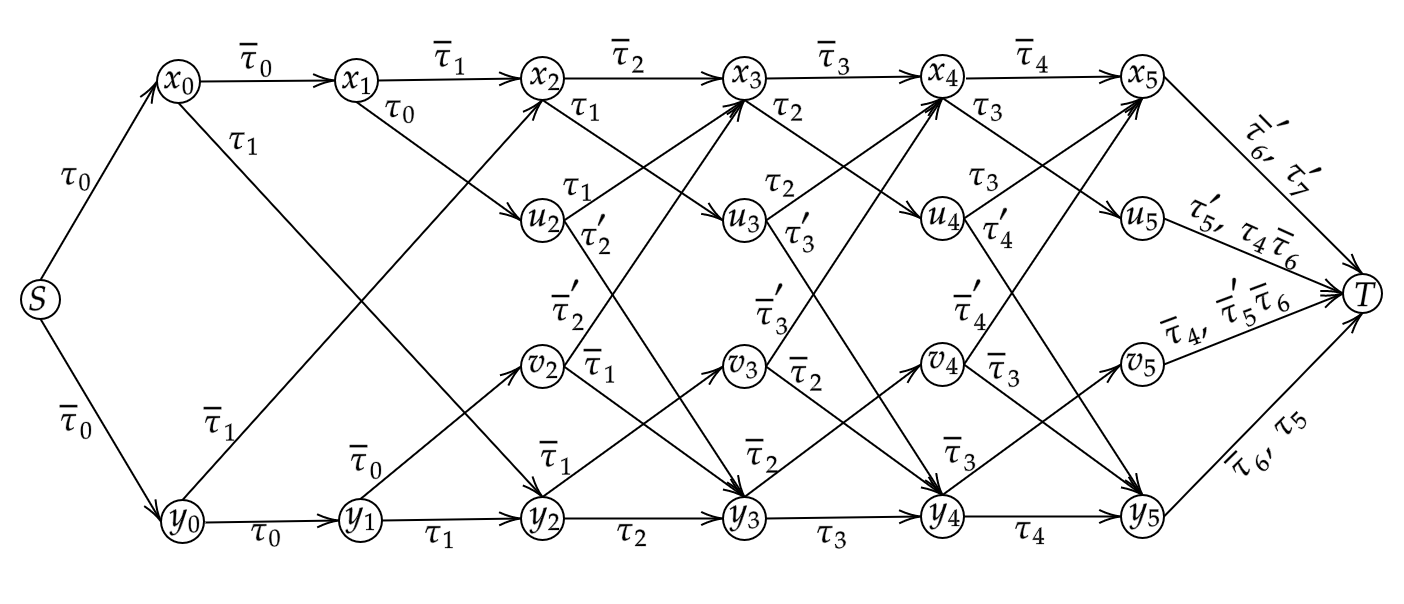
\includegraphics[natwidth=1404,natheight=604,scale=0.3]{t7.png}

More specifically, the leftmost state $S$ is the starting state and the rightmost state $T$ is the ending state. If we label the states in the first row as $x_0,x_1,\ldots,x_{n-2}$ and label the states in the last row as $y_0,y_1,\ldots,y_{n-1}$ and the middle ones are $u_2,u_3,\ldots,u_{n-2}$ and $v_2,v_3,\ldots,v_{n-2}$, the transition in each edge will be:

$x_i \overset{\overline{\tau}_{i}}{\longrightarrow} x_{i+1}, \quad x_i \overset{\tau_{i-1}}{\longrightarrow} u_{i+1}$

$y_i \overset{\tau_{i}}{\longrightarrow} y_{i+1}, \quad y_i \overset{\overline{\tau}_{i-1}}{\longrightarrow} v_{i+1}$

$u_i \overset{\tau_{i-1}}{\longrightarrow} x_{i+1}, \quad u_i \overset{\tau^\prime_{i}}{\longrightarrow} y_{i+1}$

$v_i \overset{\overline{\tau}_{i-1}}{\longrightarrow} y_{i+1}, \quad v_i \overset{\overline{\tau}^\prime_{i}}{\longrightarrow} x_{i+1}$

where $\tau_i$ is the \textit{Thue-Morse word} of order $i$, $\overline{\tau}_i$ is the inversion of $\tau_i$, $\tau^\prime_i=\overline{\tau}_{i-2}\overline{\tau}_{i-1}$, $\overline{\tau}^\prime_i$ is the inversion of $\tau^\prime_i$.

The transitions from $x_{n-2},y_{n-2},u_{n-2},v_{n-2}$ to $T$ are different:

$x_{n-2} \overset{\overline{\tau}^\prime_{n-1}}{\longrightarrow} T, \quad x_{n-2} \overset{\tau^\prime_n}{\longrightarrow} T$

$y_{n-2} \overset{\overline{\tau}_{n-1}}{\longrightarrow} T, \quad y_{n-2} \overset{\tau_{n-2}}{\longrightarrow} T$

$u_{n-2} \overset{\tau^\prime_{n-2}}{\longrightarrow} T, \quad u_{n-2} \overset{\tau_{n-3} \overline{\tau}_{n-1}}{\longrightarrow} T$

$v_{n-2} \overset{\overline{\tau}_{n-3}}{\longrightarrow} T, \quad v_{n-2} \overset{\overline{\tau}^\prime_{n-2} \overline{\tau}_{n-1}}{\longrightarrow} T$

And in addition, $T,x_{n-2},y_{n-3},x_{n-4},y_{n-5}, \ldots$ are the accepting states.

Actually, we don't need to build the whole \textit{CSAM}: only the first $O(\log |u|)$ states are enough.

We can find the corresponding state of string $u$ and find the size of the right set. The size of the right set is the number of different path ending in an accepting state, which can be calculated easily. This solves the first problem.

As for the second problem, we need to find the right set of other states. And also only $O(\log |u|)$ states are needed. Since the size of $\mathrm{Right}(x_i)$ is greater than or equal to $\mathrm{Right}(x_{i+1})$.

\end{tutorial}
